\documentclass[a4paper,10pt]{article}
\usepackage[left=1.5cm, right=1.5cm, top=1.5cm, bottom=1.5cm]{geometry}
\usepackage{enumitem}
\usepackage[hidelinks]{hyperref}
\usepackage{graphicx}
\usepackage{tikz} % circular photo
\usepackage{xcolor} % colors
\setlength{\parindent}{0pt}
\setlist[itemize]{leftmargin=*,noitemsep,topsep=0pt}

% ---------- Custom Commands ----------
% button-style link
\newcommand{\buttonlink}[2]{%
  \colorbox{gray!20}{\hyperref[#1]{\textcolor{black}{#2}}}%
}

% colored section title (no line under)
\newcommand{\cvsection}[2]{%
  \section*{\textcolor{blue!50!black}{#1}}\label{#2}%
  \vspace{4pt}%
}

\hypersetup{
  pdftitle={Curriculum Vitae - Nuzmol Islam Khan},
  pdfauthor={Nuzmol Islam Khan}
}

\begin{document}

% -------------------- Header --------------------
\begin{tabular}{@{}p{0.72\textwidth}@{}p{0.28\textwidth}@{}}
\begin{minipage}[c]{\linewidth}
    {\LARGE \textbf{Nuzmol Islam Khan}} \\[4pt]
    \href{mailto:mdnuzmolislam30@gmail.com}{mdnuzmolislam30@gmail.com} \; | \; +880-1986822599 \\
    \href{https://www.linkedin.com/in/mdnuzmol}{LinkedIn : mdnuzmol} \; | \;
    \href{https://github.com/yourgithub}{GitHub}
\end{minipage} &
\begin{minipage}[c]{\linewidth}
    \raggedleft
    \begin{tikzpicture}
        \clip (0,0) circle (1.5cm);
        \node at (0,0) {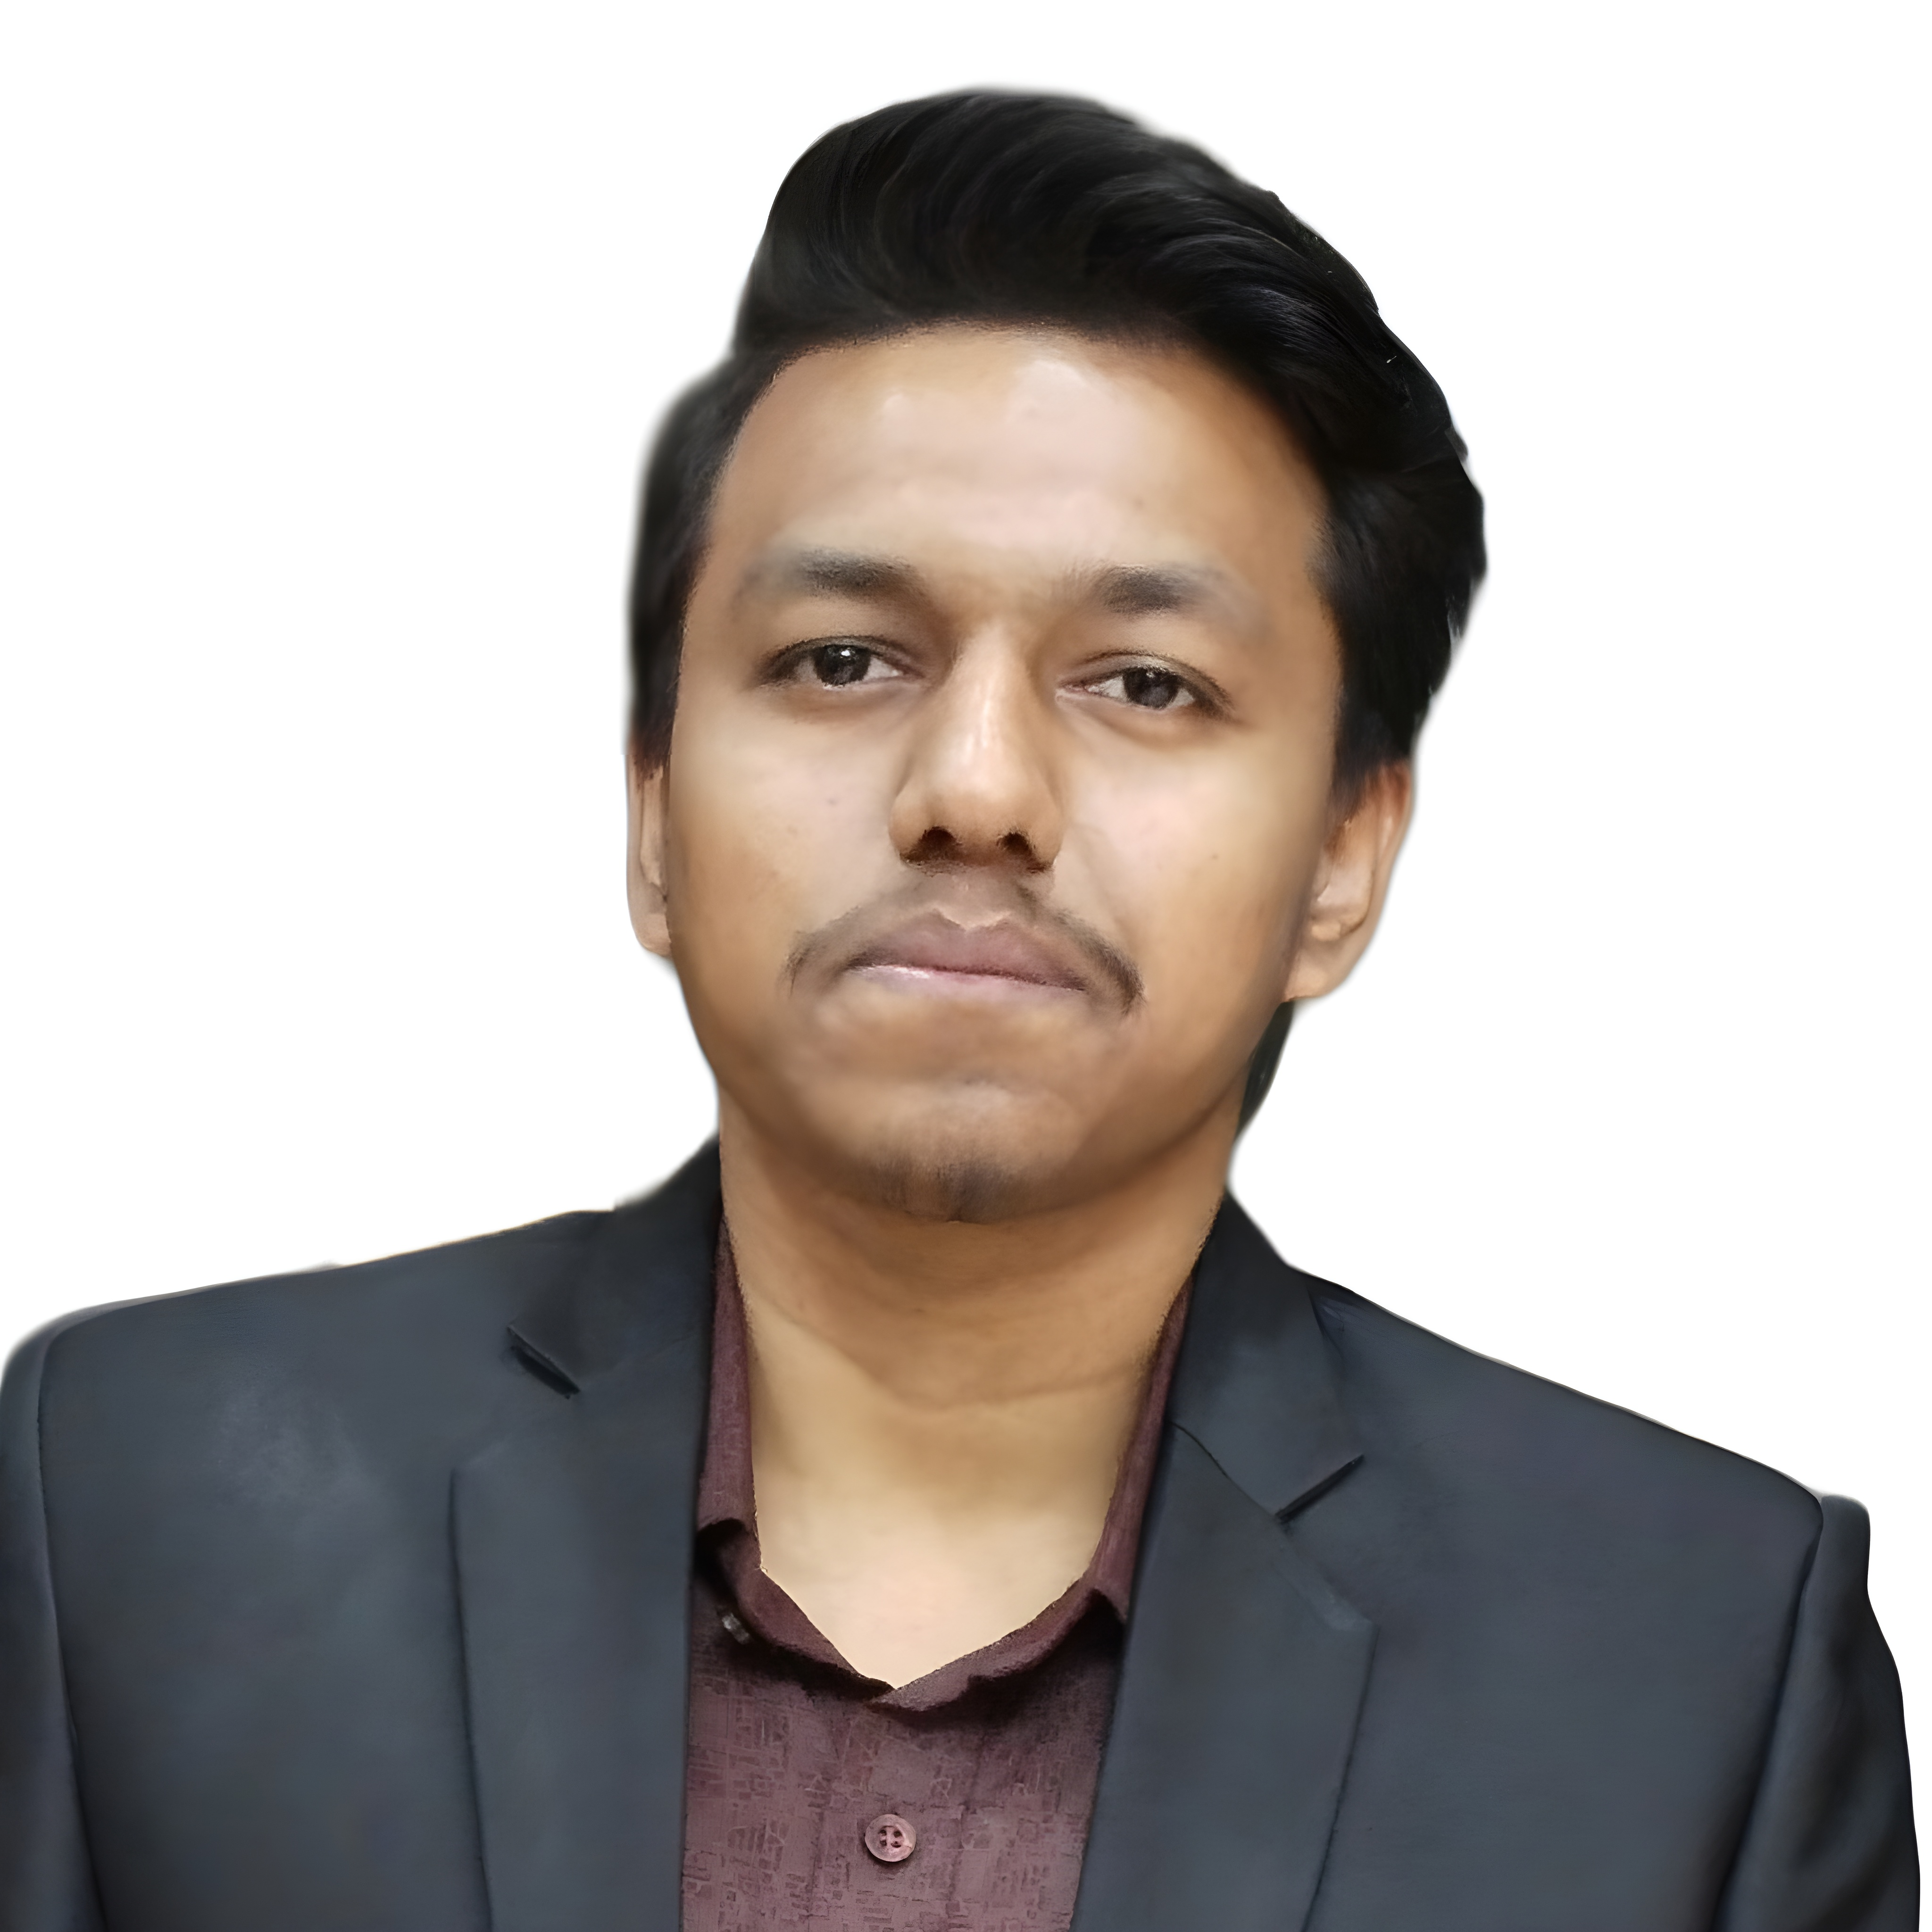
\includegraphics[width=3cm]{Profile picture.png}};
    \end{tikzpicture}
\end{minipage}
\end{tabular}

\vspace{8pt}

% -------------------- TOC Buttons --------------------
\noindent
\buttonlink{sec:summary}{Summary} \hspace{3pt}
\buttonlink{sec:skills}{Skills} \hspace{3pt}
\buttonlink{sec:projects}{Projects} \hspace{3pt}
\buttonlink{sec:experience}{Experience} \hspace{3pt}
\buttonlink{sec:education}{Education} \hspace{3pt}
\buttonlink{sec:certs}{Certifications}

\vspace{8pt}

% -------------------- Sections --------------------
\cvsection{Professional Summary}{sec:summary}
Aspiring Data Analyst and Frontend Developer with skills in Python, SQL, Excel, and web technologies (HTML, Tailwind CSS, JavaScript). Experienced in cleaning and analyzing datasets, creating interactive dashboards, and developing responsive web apps.

\cvsection{Technical Skills}{sec:skills}
\begin{tabular}{p{3.3cm} p{12cm}}
\textbf{Data:} & Python (Pandas, NumPy), SQL, Excel, Power BI, Tableau \\
\textbf{ML / Analysis:} & EDA, Feature Engineering, Clustering (K-Means), Hypothesis Testing \\
\textbf{Web:} & HTML5, CSS3, Tailwind CSS, JavaScript (ES6), Responsive Design \\
\textbf{Pro:} & HTML5, CSS3, Tailwind CSS, JavaScript (ES6), Responsive Design \\
\textbf{DB / Tools:} & MySQL, Git, LaTeX, VScode \\
\end{tabular}

\cvsection{Projects}{sec:projects}
\textbf{Sales Data Analysis Dashboard} \\
Tools: Python, Pandas, Power BI \\
Summary: Cleaned and analyzed retail sales data to reveal revenue trends and top products. Built an interactive dashboard. \\
\href{https://github.com/yourgithub/sales-dashboard}{GitHub}

\vspace{4pt}
\textbf{Customer Segmentation Web App} \\
Tools: Python, Flask, Tailwind CSS \\
Summary: Implemented K-Means clustering and built a responsive Tailwind CSS frontend. \\
\href{https://github.com/yourgithub/customer-segmentation-app}{GitHub}

\vspace{4pt}
\textbf{Portfolio Website} \\
Tools: HTML, Tailwind CSS, JavaScript \\
Summary: Created a personal portfolio to showcase projects and skills. \\
\href{https://yourwebsite.com}{Live Link}

\cvsection{Experience}{sec:experience}
\textbf{Data Analysis Intern (Optional)} \\
Company Name \; | \; Month Year -- Month Year \\
\begin{itemize}
  \item Cleaned and analyzed sales/customer datasets.
  \item Built automated reports reducing manual work.
\end{itemize}

\cvsection{Education}{sec:education}
\textbf{B.Sc. in Computer Science \& Engineering} \\
University Name, City \hfill Year -- Present

\cvsection{Certifications}{sec:certs}
\begin{itemize}
  \item Google Data Analytics Professional Certificate (Coursera)
  \item Responsive Web Design (freeCodeCamp)
  \item SQL for Data Analysis (DataCamp)
\end{itemize}



\end{document}
